%\documentclass{article}
%\documentclass[11pt,twocolumn]{article}
\documentclass[preprint,12pt,3p]{elsarticle}
\usepackage[utf8]{inputenc}
%\usepackage{authblk}

\linespread{2}
\usepackage[version=4]{mhchem}
\usepackage{pdfcomment}
\usepackage{makecell}


\date{\vspace{-5ex}}

%\usepackage[numbers,sort&compress]{natbib}
\usepackage{natbib}
%\usepackage{graphicx}
\usepackage{caption}
%\usepackage{a4wide}   %Change margins
\usepackage{multirow} %Enable merged cells in columns
\usepackage{amsmath}
\usepackage{amssymb}
\usepackage[title]{appendix}
\usepackage{indentfirst}
\usepackage[section]{placeins}

\usepackage{tikz}
\DeclareRobustCommand\fulline{\tikz[baseline=-0.6ex]\draw[thick] (0,0)--(0.5,0);}
\DeclareRobustCommand\dashedline{\tikz[baseline=-0.6ex]\draw[thick,dashed] (0,0)--(0.54,0);}

\usepackage{nomencl}
\setlength{\nomitemsep}{-\parsep}
\makenomenclature
\newcommand\Nomenclature[2]{\nomenclature[#2]{#1}{#2}}

\usepackage{etoolbox}
\renewcommand\nomgroup[1]{%
  \item[\bfseries
  \ifstrequal{#1}{A}{Abbreviantions}{%
  \ifstrequal{#1}{R}{Roman Letters}{%
  \ifstrequal{#1}{G}{Greek Letters}{%
  \ifstrequal{#1}{S}{Super/subscripts}{%
  \ifstrequal{#1}{L}{List of Symbols}{}}}}}%
]}

\usepackage[capitalise]{cleveref}

\usepackage{lineno}

\journal{Fluid Phase Equilibria}

\begin{document}

\begin{frontmatter}

\title{Renormalization Group Theory Applied to the CPA Equation of State: Impacts on Phase Equilibrium and Derivative Properties}

%\maketitle

\author[1]{Gabriel M. Silva}
\author[1]{Charlles R. A. Abreu}
\author[1,2]{Frederico W. Tavares}
\address[1]{Escola de Qu\'imica, Universidade Federal do Rio de Janeiro, Rio de Janeiro C.P. 68542, Brazil}
\address[2]{Programa de Engenharia Qu\'imica – COPPE, Universidade Federal do Rio de Janeiro, Rio de Janeiro, C.P. 68542, Brazil}

\begin{abstract}
Calculation of thermodynamic properties such as vapor-liquid phase behavior with equations of state is largely and successfully employed in chemical engineering applications.
However, in the proximities of the critical point, the different density-fluctuation scales inherent to critical phenomena introduce significant changes in these thermodynamic properties, with which the classical equations of state are not prepared to deal.
Aiming at correcting this failure, we apply a renormalization-group methodology to the CPA equation of state in order to improve the thermodynamic description in the vicinity of critical points.
We use this approach to compute vapor-liquid equilibrium of pure components and binary mixtures, as well as derivative properties such as speed of sound and heat capacity.
Our results show that this methodology is able to provide an equation of state with the correct non-classical behavior, thus bringing it in consonance with experimental observations vapor-liquid equilibrium and derivative properties in near-critical conditions.
\end{abstract}

\begin{keyword}
Renormalization \sep Cubic-Plus-Association \sep Phase Equilibrium \sep Speed of Sound \sep Heat Capacity
\end{keyword}

\end{frontmatter}

\linenumbers

%\renewcommand{\thesection}{\arabic{section}.}
\renewcommand{\thesection}{\arabic{section}}
\section{Introduction}

The development of industrial processes requires models capable of describing fluid behavior and properties with accuracy.
Equations of state are very successful tools when used to calculate thermodynamic properties of fluids far away from their critical points.
However, they fail in near-critical and critical conditions, in which fluids undergo several changes in their classical behavior \cite{sengers1986thermodynamic}.

Many unit operations in engineering involve high pressure or high temperature conditions, in which many mixtures approach critical states.
Common examples occur in natural gas processing, in which the natural gas can form mixtures with \ce{CO_2} and \ce{H_{2}S} and be found in near-critical states either at reservoir or at transport/operating conditions  \citep{kermani2003carbon}.

Experimentally, it is observed that fluids exhibit a universal non-classical behavior in the vicinity of critical points, which is evidenced in the so-called critical exponents \citep{carles2010brief}.
One theoretical explanation is that, at the critical point, the correlation length is in the order of the system size and, because only fluctuations with wavelengths below the correlation length have an expressive impact on the free energy of a fluid, long-wavelength interactions play a major role in the near-critical region.
This mechanism gives rise to fluctuations that imply significant changes to the fluids properties.
Far away from the critical point, instead, the correlation length is in the order of magnitude of the molecule diameters, thus diminishing the influence of long-range interactions and giving the short-range repulsive forces a major role.

Equations of state are commonly used to model fluids in industrial processes.
For instance, the Soave-Redlich-Kwong (SRK) \cite{soave1972equilibrium} and Peng-Robinson (PR) \cite{peng1976new} equations of state are used in a wide range of applications.
However, for some applications in which molecules are capable of making hydrogen-bonds, both equations present poor performance in representing liquid phases, both for phase equilibrium and derivative properties.
In order to overcome this limitation, Kontogeorgis \textit{et al}. \cite{kontogeorgis1996equation} combined the SRK equation of state with Wertheim's first-order thermodynamic perturbation theory (TPT-1), such as in SAFT \citep{chapman1990new}.
The resulting equation of state (Cubic-Plus-Association, CPA) is capable of representing phase equilibrium and derivative properties of pure substances and mixtures with better accuracy in states far enough from critical points.

The lack of accuracy of classical equations of state in describing thermodynamic properties in near-critical conditions is evidenced by the fact that they predict a critical exponent of $1/2$, while the value actually observed experimentally is $1/3$ \cite{sengers1974van,wyczalkowska2004critical,stanley1999scaling}.
Strategies to improve the description of critical behavior by equations of state based on reestimating parameters are somewhat common in the literature, with rather good results being achieved \cite{palma2017re,vinhal2017evaluation}.
In all cases, however, due to the nature of equations of state one cannot correct the scaling of critical phenomena by simply reestimating parameters.

The equations of state are mean-field theories by nature, and hence do not treat density fluctuations correctly as the fluid approach the critical point.
%Consequently, the critical exponents which they predict differ from those obtained from experiments.
Many theories aim at introducing non-classical behavior to equations of state.
Some methods are based on the hierarchical reference theory \cite{parola1984liquid, parola1985hierarchical, meroni1990differential, meroni1993differential}, but these have not been frequently developed and applied because of its mathematical complexity.
Another category of methods is based on a renormalized Landau expansion of the free energy \cite{wyczalkowska2004critical, chen1990crossover, kiselev1991universal, kiselev1998cubic, anisimov1992crossover, kiselev1999cubic, kiselev1999crossover}, which introduces a crossover behavior to the equations of state, turning them into non-analytical models with many adjustable parameters.
A third category of methods, developed by White and Zhang \cite{white1993renormalization, white1995renormalization, white1998renormalization}, relies on the renormalization group (RG) theory via phase space cell approximation.
This method introduces a recursive procedure intended to renormalize the free energy obtained from equations of state.
With this approach, it is possible to treat the problem of fluctuations in different scales, evolving from the microscopic scale up to the macroscopic scale in a recursive manner.
In this fashion, one is able to use common equations of state to better represent phase equilibrium and thermodynamic properties in conditions that comprehend near-critical and supercritical states.

Since its first application \citep{white1993renormalization}, White and Zhang’s recursive method has been improved by a number of authors.
The same authors, for instance, extended the range in which the method could be applied \cite{white1998renormalization}.
Lue and Prausnitz \cite{lue1998renormalization, lue1998brenormalization} and Mi \textit{et al}. \cite{mi2004improved} improved the method so that is can be applied to a large temperature range, even far away from the critical point.
Thus far, many authors have applied this method using different mean-field theories (e.g.
MSA \citep{lue1998renormalization}, equation of state for chain-like molecules \cite{jiang1999equation, jiang2000phase}, the SAFT equation and its variants \cite{llovell2004thermodynamic, forte2011application, bymaster2008renormalization, tang2010renormalization, llovell2006global, forte2013application, dias2009thermodynamic, llovell2006second, llovell2006prediction, llovell2007phase}, cubic equations \cite{xu2011prediction,xu2010crossover,pcm2017application,llovell2008accurate,qiu2006vapor,cai2006vapor,cai2004thermodynamics}, and others \cite{ghobadi2013renormalization,choi2016renormalization}), obtaining similar results.
However, some aspects in the method are still unclear, including parameter estimation procedures and approximations in the renormalization equations.
Hence, there is still need for further assessment of the method's capabilities and limitations.

The present work aims at evaluating the impacts on modeling phase equilibrium and derivative properties when applying the renormalization group theory with the CPA equation of state, referred to as the CPA+RG approach for short.
We studied several pure substances, as well as different mixtures containing \ce{CO_2} or \ce{H_{2}S}, in conditions near-to and far from the critical point.
In addition, we provide a parameter estimation procedure that improves the methodology.

This article is divided as follows.
First, we discuss briefly on the applied mean-field theory (the CPA equation of state) and the renormalization-group methodology.
This is followed by details of the numerical procedures.
Then, we present phase equilibrium results of pure substances and binary mixtures, as well as results for derivative properties such as heat capacity and speed of sound.
Finally, we present some concluding remarks.

\section{Thermodynamic Modeling}

Pure substances and binary mixtures in vapor-liquid equilibrium and at supercritical conditions were evaluated using the Cubic-Plus-Association equation of state \citep{kontogeorgis1996equation}.
In its pressure-explicit form, such equation reads
\begin{equation} \label{eq:pressure_cpa}
%P = \frac{RT}{v-b}-\frac{a}{v(v+b)}-\frac{1}{2}\frac{RT}{v} \left(1+\rho\frac{\partial \ln g}{\partial \rho}\right)\sum_{i=1}^{n_c} x_{i} \sum_{A_{i}}(1-X_{A_{i}})
P = \frac{\rho RT}{1-\rho b}-\frac{a \rho^2}{1+\rho b}-\frac{1}{2} \rho RT \left(1+\rho\frac{\partial \ln g}{\partial \rho}\right)\sum_{i=1}^{n_c} x_{i} \sum_{A_{i}}(1-X_{A_{i}})
\end{equation}
where $P$ is the pressure,
$R$ is the ideal gas constant,
%$v$ is the molar volume,
$\rho$ is the molar density,
$b$ is the mixture co-volume parameter,
$a$ is the mixture energy parameter,
$T$ is the temperature,
$g$ is the contact-value of the radial distribution function,
$n_c$ is the number of components in the mixture,
$x_{i}$ is the mole fraction of the $i$-th component,
$A_{i}$ is the association site $A$ of the $i$-th component, and
$X_{A_{i}}$ is the fraction of non-associated type-$A$ sites of the $i$-th component.
As the renormalization procedure provides corrections explicitly to the Helmholtz free energy density, it is useful to represent the CPA equation of state in its Helmholtz-explicit form, given by
%\begin{subequations}
\begin{equation} \label{eq:helm_res_cpa}
\bar{a}_\text{CPA}^\text{res} =\bar{a}_\text{SRK}^\text{res} + \bar{a}_\text{assoc}^\text{res},
\end{equation}
where
\begin{equation} \label{eq:helm_res_srk}
\bar{a}_\text{SRK}^\text{res} = -RT\ln(1-\rho b)-\frac{a}{b}\ln(1+\rho b)   
\end{equation}
and
\begin{equation} \label{eq:helm_res_assoc}
\bar{a}_\text{assoc}^\text{res} = RT\sum_{i=1}^{n_c} x_{i} \sum_{A_{i}}\left(\ln X_{A_{i}} - \frac{X_{A_{i}}}{2} + \frac{1}{2}\right).
\end{equation}
%\end{subequations}

In these equations, $\bar{a}^\text{res}$ is the residual molar Helmholtz free energy.
The mixture parameters $a$ and $b$ are calculated using the van der Waals one-fluid mixing rule with the classical combining rules, that is,
\begin{equation}
a = \sum_{i=1}^{n_c} \sum_{j=1}^{n_c} x_{i}x_{j}\sqrt{a_{i}a_{j}}(1-k_{ij})
\end{equation}
and
\begin{equation}
b = \sum_{i=1}^{n_c}x_{i}b_{i},
\end{equation}
where $k_{ij}$ is a binary interaction parameter (here considered as zero for all examples).
The energy parameter of each component, $a_{i}$, is calculated using a Soave-type temperature dependency,
\begin{equation}
a_{i}(T) = a_{0_{i}}\left[1+c_{1_{i}}\left(1-\sqrt{\frac{T}{T_{c_{i}}}}\right)\right]^2,
\end{equation}
where $a_{0_{i}}$, $b_{i}$, $c_{1_{i}}$ are parameters of the CPA equation.
The last term of Eq.~\ref{eq:pressure_cpa} is the association term, in which $X_{A_{i}}$ represents the fractions of non-associated type-$A$ sites of the \textit{i}-th component, calculated by
\begin{equation} \label{eq:frac_nb}
X_{A_{i}} = \left(1+\rho \sum_{j=1}^{n_c} x_{j} \sum_{B_{j}} X_{B_{j}} \Delta^{A_{i}B_{j}}\right)^{-1},
\end{equation}
in which $\Delta^{A_{i}B_{j}}$ is the association strength, given by
\begin{equation} \label{eq:delta_cpa}
\Delta^{A_{i}B_{j}} = g(\rho)\left[\exp\left(\frac{\epsilon^{A_{i}B_{j}}}{RT}\right)-1\right]b_{ij}\beta^{A_{i}B_{j}},
\end{equation}
with $b_{ij} = \frac{b_{i}+b_{j}}{2}$ and where $\beta_{i}^{A_{i}B_{j}}$ and $\epsilon_{i}^{A_{i}B_{j}}$ are the association parameters of the CPA equation, $g(\rho)$ is the contact-value of the radial distribution function. Here we employ the approximate hard-sphere expression $g(\rho) = \frac{1}{1-1.9\eta}$, where $\eta = \frac{b\rho}{4}$ is the packing fraction.

Thus, the version of the CPA equation presented here is the one commonly referred to in the literature as simplified CPA (s-CPA) \citep{kontogeorgis1999multicomponent}. However, we will simply use the term CPA for simplicity.
In this work, $X_{A_{i}}$ is calculated following the numerical procedure proposed by Michelsen \textit{et al}. \cite{michelsen2006robust}.

The recursive method developed by White and Zhang \cite{white1993renormalization, white1995renormalization, white1998renormalization} and by Salvino and White \citep{salvino1992calculation} introduces density fluctuations to a specified grid of Helmholtz energy density.
The method is based on the phase space cell approximation developed by Wilson \cite{wilson1971renormalization, wilson1971brenormalization}, where each iteration accounts for fluctuations of longer and longer wavelengths.
This introduces a non-analytic correction to the analytical equation of state.
An illustration of the method is represented in Fig.~\ref{fig:schematics}.

\begin{figure}[h!]
\centering
\captionsetup{justification=centering}
\makebox[\textwidth][c]{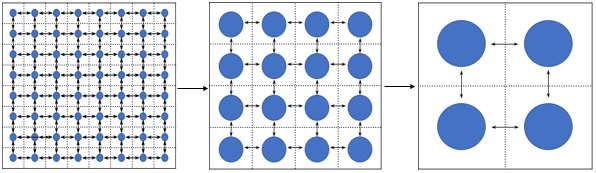
\includegraphics[width=1.0\textwidth]{figures/renorm_schematics.png}}
\caption{Schematics of the phase space cell approximation. First, interactions between molecules are calculated with a mean-field theory. Next, fluctuations are included and \hl{nearby molecules are considered to form clusters which behave as single entities. Then, iterations are then carried out until.......}}
\label{fig:schematics}
\end{figure}

The renormalization group theory as introduced by White and co-workers \cite{white1993renormalization,white1995renormalization,white1998renormalization} and further developed by Lue and Prausnitz \cite{lue1998renormalization, lue1998brenormalization} is based on a transformation of the grand canonical partition function into a functional integral.
To note, in this work we used the derivation provided by White and co-workers \cite{white1993renormalization,white1995renormalization,white1998renormalization}, and applied successfully by other authors for cubic-EoS \cite{cai2006vapor,pcm2017application,xu2010crossover,xu2011prediction}, details of the method can be found in these works.
To briefly address the method, the interaction potential $u(r)$ is considered to be divided into two main contributions, a reference term (related to short-range repulsions) and a perturbation term (related to long-range attractive interactions)
Considering that the repulsive part of the potential accounts only for very-short-wavelength fluctuations and that the perturbation part takes into account both short- and long-wavelength fluctuations, the renormalization method is applied only to the attractive part.
Mean-field theories are then used because we consider then to provide a good approximation for the short-range repulsions and fluctuations smaller than a given cutoff length $L$.

As we are concerned only with the attractive part, in order to apply the renormalization method we need to subtract the attractive potential already included in the mean-field solution, considering it to be a bad approximation, since the mean-field theory cannot deal accurately with long-wavelength fluctuations.
This leads to the approximation
\begin{equation} \label{eq:f01}
f_{0}(\rho) = f^{EoS} + \alpha\rho^2,
\end{equation}
where $f^\text{EoS}$ is the Helmholtz free energy density calculated using the mean-field theory (in this work, the CPA equation of state), and $\alpha$ is the interaction volume, in units of \hl{$energy*volume/mol^{2}$}, given by

\begin{equation} \label{eq:alphav}
\alpha = -\frac{1}{2} \int u_\text{att} dr,
\end{equation}
where $u_\text{att}$ is the attractive part of the potential.
Since there is no explicit potential for the CPA equation of state, considering previous work with both the SRK and CPA equations of state \cite{cai2004thermodynamics, pcm2017application, xu2010crossover}, the attractive part of the potential is correlated to half of parameter $a$, which here is considered as an approximation to the contribution of the attractive part of the potential (divided by the volume) to the Helmholtz free energy density.
This leads us to

\begin{equation} \label{eq:arho2}
\alpha\rho^2 = \frac{1}{2}a\rho^2.
\end{equation}

The Helmholtz free energy corresponding to the zero-order solution ($f_{0}$) is given by the mean-field theory result subtracted by the approximated attractive term.
Combining \cref{eq:helm_res_cpa,eq:f_to_a,eq:f01,eq:arho2}, the Helmholtz free energy density zero-order solution is
\begin{equation} \label{eq:f00}
f_{0}(\rho) = \rho RT\ln\left(\frac{\rho}{1-\rho b}\right)-\frac{a\rho}{b}\ln(1+\rho b) + \rho RT\sum_{i=1}^{n_c} x_{i} \sum_{A_{i}}\left(\ln X_{A_{i}} - \frac{X_{A_{i}}}{2} + \frac{1}{2}\right) + \frac{1}{2} a\rho^2.
\end{equation}  

The phase space cell approximation method consists in adding the effect of long-range fluctuations through recursive steps, thus correcting the influence of the long-range interactions on the Helmholtz free energy density of the mean-field solution.
In this work, the equation derived from the procedures above and used to calculate these corrections is
\begin{equation} \label{eq:fn}
f_{n}(\rho) = df_{n}(\rho) + f_{n-1}(\rho),
\end{equation}
with $df_{n}(\rho)$ being the change in Helmholtz free energy density at iteration $n$, given by
\begin{equation} \label{eq:dfn}
df_{n}(\rho) = -K_{n} \ln\left[\frac{\Omega_{n}^{s}(\rho)}{\Omega_{n}^{l}(\rho)}\right],
\end{equation}
where $K_{n} = \frac{k_{b}T}{(2^{n}L)^3}$, with $k_{b}$ being the Boltzmann constant,
$\Omega_{n}^{s}$ is the density of short-wavelengths fluctuations, and
$\Omega_{n}^{l}$ is the density of long-wavelengths fluctuations.
These can be obtained from
\begin{equation} \label{eq:Omega}
\Omega_{n}^{\gamma} = \int_{0}^{\min(\rho,\rho_{\max}-\rho)}\exp\left[-\frac{G_{n}^{\gamma}(\rho,x)}{K_{n}}\right]dx \qquad  \gamma = s,l
\end{equation}
with
\begin{equation} \label{eq:Gn}
G_{n}^{\gamma}(\rho) = \frac{f_{n}^{\gamma}(\rho+x)-2f_{n}^{\gamma}(\rho)+f_{n}^{\gamma}(\rho-x)}{2} \qquad \gamma = s,l,
\end{equation}
where $f_{n}^{s}$ and $f_{n}^{l}$ are the modified Helmholtz free energy terms related to short-wavelength and long-wavelength fluctuations, respectively.
They are computed by

\begin{equation} \label{eq:fns_battle}
f_{n}^{s} = f_{n-1} + \frac{\alpha \rho^2}{2^{2n}}\left(\frac{\psi w^2}{2L^2}\right)
\end{equation}
and
\begin{equation} \label{eq:fnl}
f_{n}^{l} = f_{n-1} + \alpha\rho^2,
\end{equation}
where $w$ is the range of the attractive potential, $psi$ is the average gradient of the wavelet chosen for renormalization, which doesn't depends on the interaction potential.
Since the attractive potential for the CPA EoS is not clear, we followed other authors in considering the whole term $\left(\frac{\psi w^2}{2L^2}\right)$ in \cref{eq:fns} as an adjustable parameter $phi$, leading to

\begin{equation} \label{eq:fns}
f_{n}^{s} = f_{n-1} + \frac{\alpha \rho^2 \phi}{2^{2n}}
\end{equation}

The final Helmholtz free energy density is calculated as

\begin{equation} \label{eq:ff}
f = \lim_{n \rightarrow \infty} f_{n} - \alpha\rho^2.
\end{equation}

The term $-\alpha\rho^2$ in \cref{eq:ff} is included since we want to recover the fluids original behavior far away from the critical point, because in this condition $\lim_{n \rightarrow \infty} f_{n}$ tends to zero.
It is important to note that other authors \cite{llovell2004thermodynamic,llovell2006global,llovell2006prediction,bymaster2008renormalization,tang2010renormalization}, following more closely the modifications suggested by Lue and Prausnitz \cite{lue1998brenormalization}, modify \cref{eq:f01,eq:ff}, which are calculated as

\begin{equation} \label{eq:f022}
f_{0}(\rho) = f^{EoS},
\end{equation}

and

\begin{equation} \label{eq:ff2}
f = \lim_{n \rightarrow \infty} f_{n}.
\end{equation}

These modifications are made when the saddle-point approximation is used within the method derivation (details are given in the work of Lue and Prausnitz \cite{lue1998brenormalization}).
In literature, these approximations were used mainly with SAFT family of EoS, not being used with cubic-EoS, still, successful results were obtained in the latter case.
This way, we chose to apply \cref{eq:f01,eq:ff} instead of \cref{eq:f022,eq:ff2} in this work.

Here we considered five iterations to converge the renormalization method (based on results to be presented on \cref{sec:pure-substance phase equilibrium results}).
To apply the renormalization procedure to mixtures, two major modifications were made.
First, the isomorphic approximation \citep{fisher1968renormalization} was used instead of the phase space cell approximation.
The main difference between the two approximations is that the former considers that the total density of the fluid is used to consider fluctuations, while the latter implies that each individual component in the mixture fluctuates independently.
Second, although the isomorphism assumption requires the chemical potential be the isomorphic variable in the present case, this is not a common independent variable for mixture phase equilibrium modeling.
Thus, following Kiselev and Friend \citep{kiselev1999cubic}, we used mole fractions as isomorphic variables instead of the individual chemical potentials.
These two approximations make possible to extend \cref{eq:f00,eq:fn,eq:dfn,eq:Omega,eq:Gn,eq:fns,eq:fnl} by simply defining mixing rules for the renormalization parameters, which are
\begin{equation} \label{eq:mix_L}
L = \sum_{i=1}^{n_c}x_{i}L_{i}^{3}
\end{equation}
and
\begin{equation} \label{eq:mix_phi}
\phi = \sum_{i=1}^{n_c}x_{i}\phi_{i}.
\end{equation}

Other authors have used these approximations within the White and Zhang approach \cite{white1993renormalization} and obtained good results \cite{cai2004thermodynamics, llovell2006global, sun2005application, pcm2017application, xu2011prediction}.
Tang and Gross \citep{tang2010renormalization} compared the phase space cell approximation and isomorphic approximation using the PC-SAFT equation of state, and concluded that both present similar performances.

The substances analyzed here are n-butane, n-octane, methanol, ethanol, \ce{CO_2}, and \ce{H_{2}S}.
These substances were chosen because of the different associative combinations that could be evaluated.
n-Butane and \ce{CO_2} were considered as non-associative substances, while methanol, ethanol, and \ce{H_{2}S} are considered as associative ones.
There is a large discussion on the literature on the most adequate associating models and considerations to represent these substances, mainly \ce{CO_2} \citep{bjorner2016modeling} and \ce{H_{2}S} \citep{ruffine2006represent}.
A common example is whether \ce{CO_2} should actually be considered as an associating molecule and, furthermore, whether the extent of quadrupole forces is important \cite{tsivintzelis2011modeling,bjorner2016modeling}.
As to diminish the influence of considered forces upon the renormalization procedure, we choose to consider \ce{CO_2} as non-associative, since we consider it to be a good approximation.
Quadrupole forces are not considered in this work for \ce{CO_2} because we believe they deserve a special attention due its nature, which is not the scope of this work.

The parameters for all substances are summarized in \cref{table:CPA_parameters}.
For all cases, the \mbox{CR-1} combination rule is considered for the association parameters (comprised of arithmetic mean for the cross-association energy and geometric mean for the cross-association volume), because of its success in a good range of applications \cite{folas2005application,folas2006application,kontogeorgis2006ten1,kontogeorgis2006ten2}.
Cross-association is considered in cases where both substances are associating ones.
The critical properties for each substance are shown in \cref{table:crit_exp}.
The terminology for the association models follows that of Huang and Radosz \cite{huang1990equation}.

\begin{table}[h!]
\centering
\caption{Parameters of the CPA equation of state used in this work.}
\label{table:CPA_parameters}
\makebox[\textwidth]{\begin{tabular}{ccccccc}
\hline
Substance   & \thead{Association\\Model} & \thead{$a_{0_{i}}$\\($Pa.m^{6}.mol$)} & \thead{$b_{i}$\\($10^{5} \, m^{3}.mol^{-1}$)} & $c_{1_{i}}$  & \thead{$\epsilon_{i}^{A_{i}B_{j}}$\\($MPa.m^{3}.mol^{-1}$)} & $\beta_{i}^{A_{i}B_{j}}$  \\ \hline
n-Butane& n.a.
 & 1.29& 7.21 & 0.70771 & -& -  \\
Methanol& 2B& 0.405   & 3.098& 0.43102 & 0.024591 & 0.0161 \\
Ethanol & 2B& 0.867   & 4.911& 0.7369  & 0.021532 & 0.008  \\
\ce{CO_2}   & n.a.
 & 0.351   & 2.72 & 0.7602  & -& -  \\
\ce{H_{2}S} & 4C& 0.32& 2.93 & 0.82805 & 0.00146  & 0.486  \\ \hline 
\end{tabular}}
\raggedright n.a.
= non-associative
\end{table}

\begin{table}[h!]
\centering
\caption{Experimental critical data obtained from NIST database \cite{nistfluids} and used as reference}
\label{table:crit_exp}
\makebox[\textwidth]{\begin{tabular}{cccc}
   \hline
Substance   & $T_{c}$ ($K$) & $P_{c}$ ($MPa$) & $\rho_{c}$ ($mol/m^{3}$)  \\ \hline
n-Butane& 425.2  & 3.797& 3920  \\
Methanol& 512.6  & 8.096& 8510  \\
Ethanol & 514.0  & 6.384& 6000  \\
\ce{CO_2}   & 304.2  & 7.382& 10600 \\
\ce{H_{2}S} & 373.4  & 8.960& 10200 \\ \hline 
\end{tabular}}
\end{table}

For every substance, after estimation of parameters L and $\phi$ (such as described in \cref{sec:Parameter Estimation}) and calculation of the vapor-liquid phase envelope, the critical exponent $\beta$ was evaluated using a linear regression from
\begin{equation} \label{eq:beta_law}
\ln\left|\frac{\rho_\text{liq}-\rho_\text{vap}}{\rho_{c}}\right| = \beta \ln\left|\frac{T-T_{c}}{T_{c}}\right|+\text{const.} \qquad (T \rightarrow T_{c}).
\end{equation}

\section{Numerical Procedures}

After defining a grid of densities (and mole fractions, in the case of mixtures), the Helmholtz free energy density is calculated at all points.
Then, \cref{eq:f00,eq:fn,eq:dfn,eq:Omega,eq:Gn,eq:fns,eq:fnl} are applied and iterations are carried out until no further change is observed to the free energy at every point ($df_{n}(\rho) \cong 0$).
Here, 5 iterations have been observed as sufficient to reach convergence in a grid of 500 density points.
Such number of points is enough for all calculations presented here.
Other authors considered even fewer density grid points (400, or even 200) \cite{cai2004thermodynamics}.
These numbers of steps and grid points were tested in preliminary studies (see \cref{fig:dfn,fig:PV_evol}).

The renormalized results of Helmholtz free energy density as a function of molar density was interpolated using cubic splines (or bicubic splines in the case of binary mixtures) and their derivatives were used to calculate variables of interest in the vapor-liquid phase equilibrium, such as chemical potential and pressure.
Details of equations and algorithms are given in Appendices \ref{app:pure substances} and \ref{app:mixtures}.

As mentioned in the previous section, the total molar density of a mixture is considered for calculating fluctuations (the isomorphism assumption) while mole fractions are used as independent variables.

Upon analyzing and determining the parameters related to the renormalization method for pure substances, phase equilibrium calculations for binary mixtures were carried out at a number of different conditions (both subcritical and critical) using the isofugacity method.

\section{Parameter Estimation}
\label{sec:Parameter Estimation}

Both parameters related to the renormalization, $L$ and $\phi$, were considered to be adjustable.
Therefore, they were obtained by fitting densities and vapor pressures to experimental data using a single objective function, given by
\begin{equation}   \label{eq:OF}
%O.F.=\sum_{i=1}^{n_{exp}} \left(\frac{\rho_{i}^{liq,exp}-\rho_{i}^{liq,calc}}{\rho_{i}^{liq,exp}}\right)^2 + \sum_{i=1}^{n_{exp}} \left(\frac{\rho_{i}^{vap,exp}-\rho_{i}^{vap,calc}}{\rho_{i}^{vap,exp}}\right)^2 + \sum_{i=1}^{n_{exp}} \left(\frac{P_{i}^{sat,exp}-P_{i}^{sat,calc}}{P_{i}^{sat,exp}}\right)^2
O.F.=\sum_{i=1}^{n_\text{exp}}\left[ \left(\frac{\rho_{i}^\text{liq,exp}-\rho_{i}^\text{liq,calc}}{\rho_{i}^\text{liq,exp}}\right)^2 + \left(\frac{\rho_{i}^\text{vap,exp}-\rho_{i}^\text{vap,calc}}{\rho_{i}^\text{vap,exp}}\right)^2 + \left(\frac{P_{i}^\text{sat,exp}-P_{i}^\text{sat,calc}}{P_{i}^\text{sat,exp}}\right)^2\right].
\end{equation}

Saturation pressure, saturated vapor density, and saturated liquid density were used in the temperature range from near-critical conditions to the critical point ($T_r=0.98$ to $T_r=1.0$).
Both liquid and vapor densities were included.
Many different approaches were used in the literature (a good review on this subject can be found in Bymaster \textit{et al}. \cite{bymaster2008renormalization}) to estimate these parameters, however, as to have a first evaluation of both parameters for the CPA EoS, we decided to fit both parameters.

A Particle Swarm Optimization algorithm was used to find the minimum of the objective function.
The obtained parameters are summarized in \cref{table:renorm_param}.

\begin{table}[ht!]
	\centering
	\caption{Renormalization method parameters estimated using the procedure described in \cref{sec:Parameter Estimation}.}
	\label{table:renorm_param}
	\makebox[\textwidth]{
		\begin{tabular}{lll}
			\hline
			Substance   & L ($\AA$) & $\phi$   \\ \hline
			n-Butane& 6.16  & 1.96  \\
			Methanol& 5.50  & 0.60  \\
			Ethanol & 5.48  & 0.75  \\
			\ce{CO_2} & 4.44  & 2.62 \\
			\ce{H_{2}S} & 4.30  & 2.40 \\ \hline 
		\end{tabular}
	}
\end{table}

\section{Results}

\subsection{Pure-Substance Phase Equilibrium}
\label{sec:pure-substance phase equilibrium results}

To define the number of iterations required for convergence, we analyzed the evolution of pure substance vapor-liquid phase envelope and the $df_{n}$ for the whole density range.
From \cref{fig:dfn,fig:PV_evol}, from our results, we observed that after the fifth iteration, the calculated $df_{n}$ for the whole density range was in the order of $10^{-15}$, thus, we considered the method as converged.
To be conservative and by following other authors  \cite{llovell2004thermodynamic, cai2004thermodynamics, pcm2017application}, the final Helmholtz free energy density we adopt here is $f_{5}$.

\begin{figure}[h!]
\centering
\captionsetup{justification=centering}
\makebox[\textwidth][c]{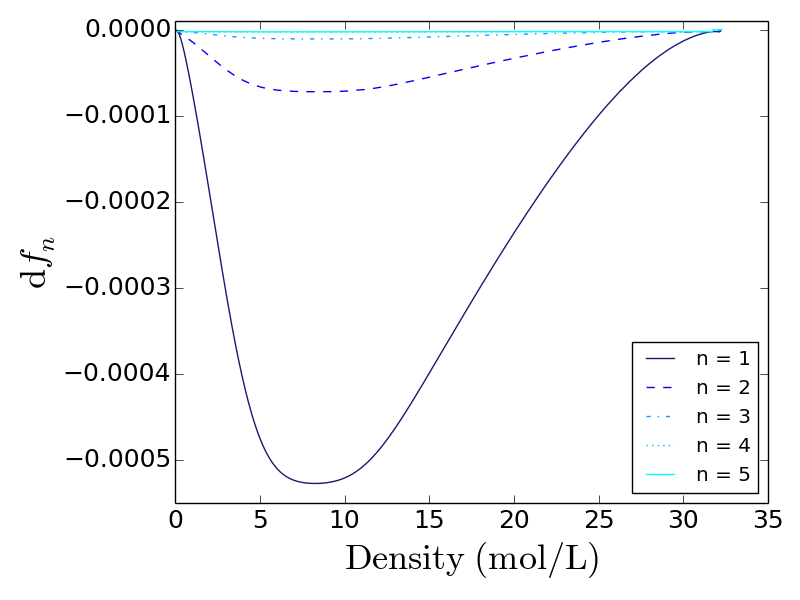
\includegraphics[width=0.65\textwidth]{figures/df_csv.png}}
\caption{Helmholtz-free energy density corrections at each iteration of the renormalization method using the CPA+RG equation of state for methanol at 512.6~K.}
\label{fig:dfn}
\end{figure}

\begin{figure}[h!]
\centering
\captionsetup{justification=centering}
\makebox[\textwidth][c]{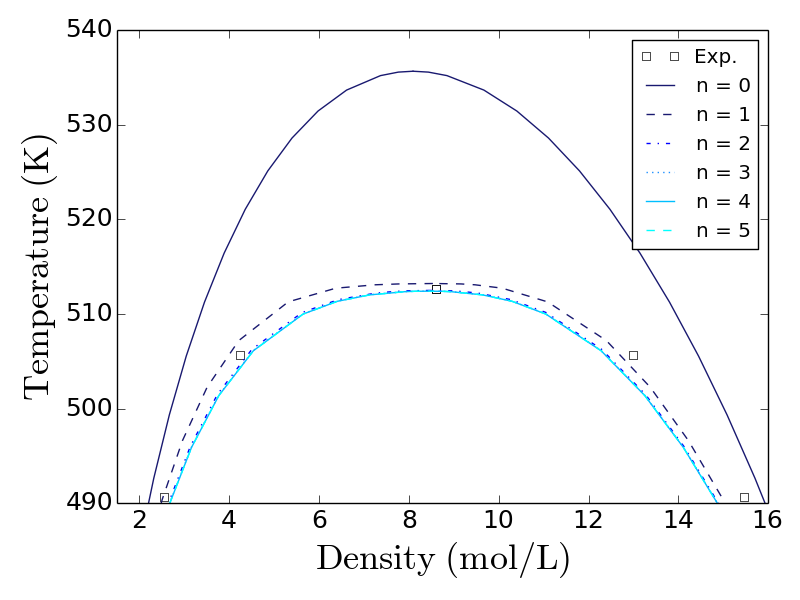
\includegraphics[width=0.65\textwidth]{figures/PV_evol.png}}
\caption{Vapor-liquid phase equilibrium envelope for methanol with CPA+RG at consecutive iterations of the renormalization method.}
\label{fig:PV_evol}
\end{figure}

Results concerning phase equilibrium calculations are summarized in \cref{fig:pure_LV,fig:sat_p,fig:crit_exp,fig:pure_isotherm,table:AAD_crit}.

\begin{figure}[h!]
\centering
\captionsetup{justification=centering}
\makebox[\textwidth][c]{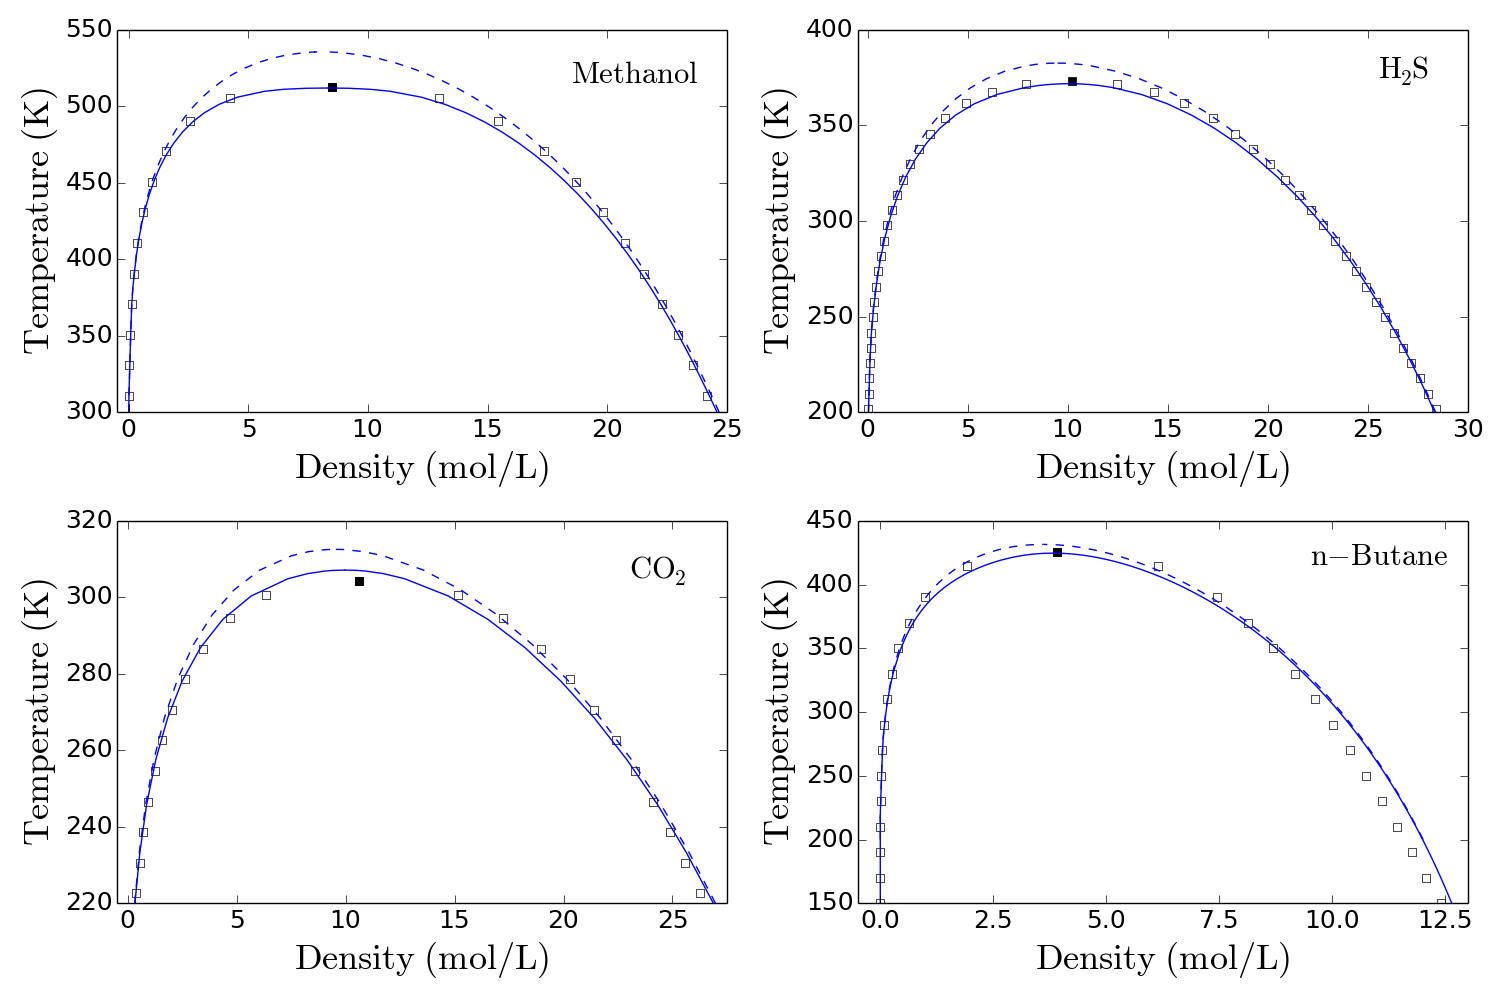
\includegraphics[width=1.0\textwidth]{figures/PV_pure_4.png}}
\caption{Vapor-liquid phase equilibrium envelope obtained for several substances.
Lines are obtained from calculations with the CPA+RG (\fulline) and CPA (\dashedline) methods.
Experimental data (symbols) were extracted from the NIST database \cite{nistfluids}.}
\pdfcomment[author=Charlles]{Problemas com esta figura:
	2) Onde estão os resultados para etanol?
}
\label{fig:pure_LV}
\end{figure}

\begin{figure}[h!]
\centering
\captionsetup{justification=centering}
\makebox[\textwidth][c]{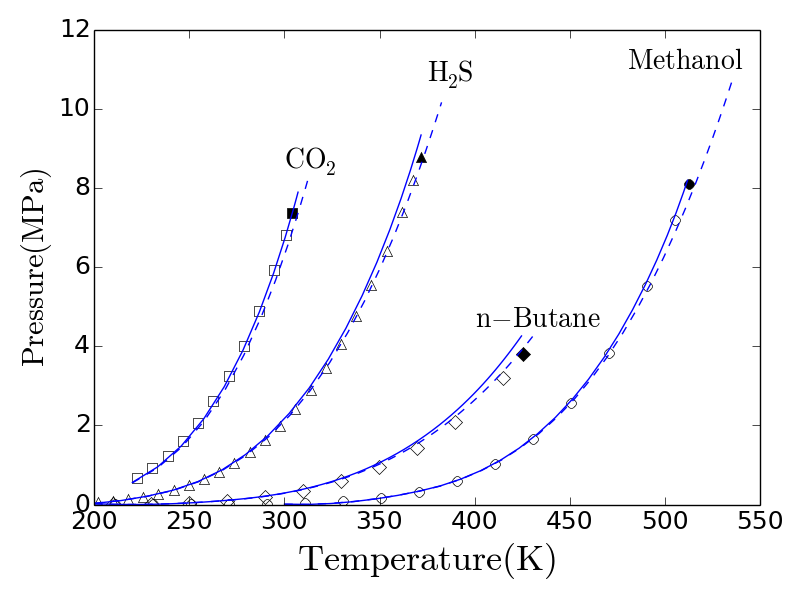
\includegraphics[width=0.65\textwidth]{figures/sat_p.png}}
\caption{Saturation pressure curves.
Lines are obtained from calculations with the CPA+RG (\fulline) and CPA (\dashedline) methods.
Experimental data (symbols) were extracted from the NIST database \cite{nistfluids}, with critical points being represented by filled symbols.}
\label{fig:sat_p}
\end{figure}

\begin{figure}[h!]
\centering
\captionsetup{justification=centering}
\makebox[\textwidth][c]{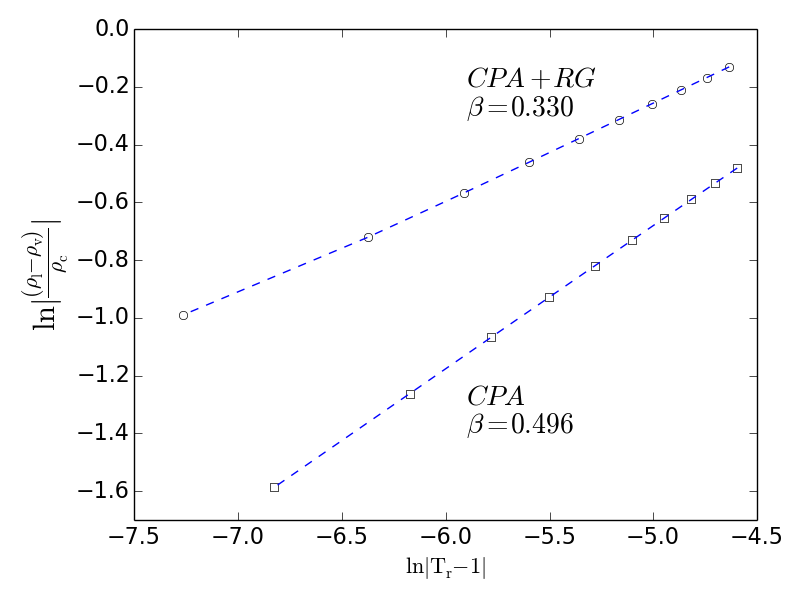
\includegraphics[width=0.65\textwidth]{figures/beta.png}}
\caption{Critical exponent calculation for methanol, resulting in $\beta = 0.330$ with CPA+RG and $\beta =0.496$ with CPA.
Symbols are obtained from calculations with the CPA+RG ($\circ$) and CPA ($\square$) methods.
Lines (\dashedline) were obtained by linear regression.
The value of $\beta$ obtained from CPA+RG is very close to the experimental value.}
\label{fig:crit_exp}
\end{figure}

\begin{figure}[h!]
\centering
\captionsetup{justification=centering}
\makebox[\textwidth][c]{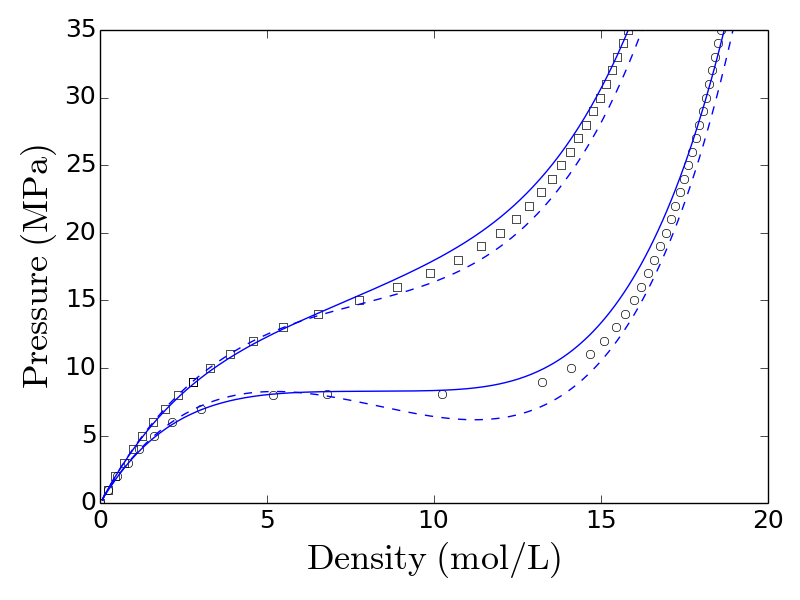
\includegraphics[width=0.65\textwidth]{figures/isotherm.png}}
\caption{Isotherms for methanol at $T_r=1.0$ (below) and $T_r=1.1$ (above).
Experimental data (symbols) were extracted from the NIST database \cite{nistfluids}.
Lines were obtained from calculations with the CPA+RG (\fulline) and CPA (\dashedline) methods.}
\label{fig:pure_isotherm}
\end{figure}

\begin{table}[h!]
\centering
\caption{Relative deviations (\%) of calculated critical points with respect to experimental data.
}
\label{table:AAD_crit}
\begin{tabular}{cccccccl} \hline
\multirow{2}{*}{Substance} & \multicolumn{2}{c}{$\displaystyle \left(100\frac{T_{c}-T_{c}^\text{exp}}{T_{c}^\text{exp}}\right)$} & \multicolumn{2}{c}{$\displaystyle \left(100\frac{P_{c}-P_{c}^\text{exp}}{P_{c}^\text{exp}}\right)$} & \multicolumn{2}{c}{$\displaystyle \left(100\frac{\rho_{c}-\rho_{c}^\text{exp}}{\rho_{c}^\text{exp}}\right)$} &  \\ \cline{2-7}
   & CPA& CPA+RG  & CPA   & CPA+RG& CPA & CPA+RG   &  \\ \hline
n-Butane   & 1.49   & 0.85& 13.54 & 6.32  & 8.01& 7.14 &  \\
Methanol   & 4.49   & -0.26& 32.68 & 0.24  & 5.17& -1.51 &  \\
Ethanol& 4.77   & 0.26 & 29.79 & 1.23  & 7.52& 1.63 &  \\
\ce{CO_2}   & 1.91   & 0.09& 11.25 & 7.26  & 9.82& -4.53 &  \\
\ce{H_{2}S}& 3.21   & -0.41& 19.79 & 4.26 & 2.96& -1.31 &  \\ \hline
\end{tabular}
\end{table}

\cref{fig:crit_exp} shows that the CPA+RG presents a critical exponent closer to the universal experimental value ($\beta = 0.330$), while the CPA equation of state presents a classical mean-field value of $\beta \sim 0.496$.

It is clear from \cref{fig:pure_LV,fig:sat_p} that the correction of the behavior of the fluid in the phase envelope when the conditions are near the critical region, leading to an asymptotic behavior at the critical point.
As conditions become farther away from the critical point, the differences between the CPA equation of state and the CPA+RG become insignificant.
This result is expected due the fact that long-wavelength fluctuations at this point are less important, and then the renormalization method does not imply any changes into the Helmholtz energy.

\cref{fig:pure_isotherm} shows the change in phase equilibrium modeling at critical and supercritical isotherms.
The CPA+RG approach is able to better predict the fluids phase behavior, because the CPA equation of state overpredicts the critical point, it describes a binary vapor-liquid phase up to its erroneous critical point, while the CPA+RG approach already describes the fluid as supercritical.
The changes in free energy for supercritical isotherm are lesser than those for critical isotherm.
In \cref{fig:sat_p} it is clear that the renormalization method has a tendency to overestimate pressure.

\cref{table:AAD_crit} shows that the errors from CPA+RG approach are smaller than the CPA equation of state, which overestimates the critical point.

\subsection{Binary Mixture Phase Equilibrium}

In all binary mixtures, we evaluated both subcritical and critical conditions for three kinds of mixture: 2 non-associating components (\ce{CO_2} + n-butane); 1 associating and 1 non-associating component (\ce{H_{2}S} + \ce{CO_2}); 2 associating components (\ce{H_{2}S} + Methanol).
In all cases the CR-1 combining rule is used.
Solvating phenomena is not considered for the case of \ce{H_{2}S} + \ce{CO_2}.

\begin{figure}[h!]
\centering
\captionsetup{justification=centering}
\makebox[\textwidth][c]{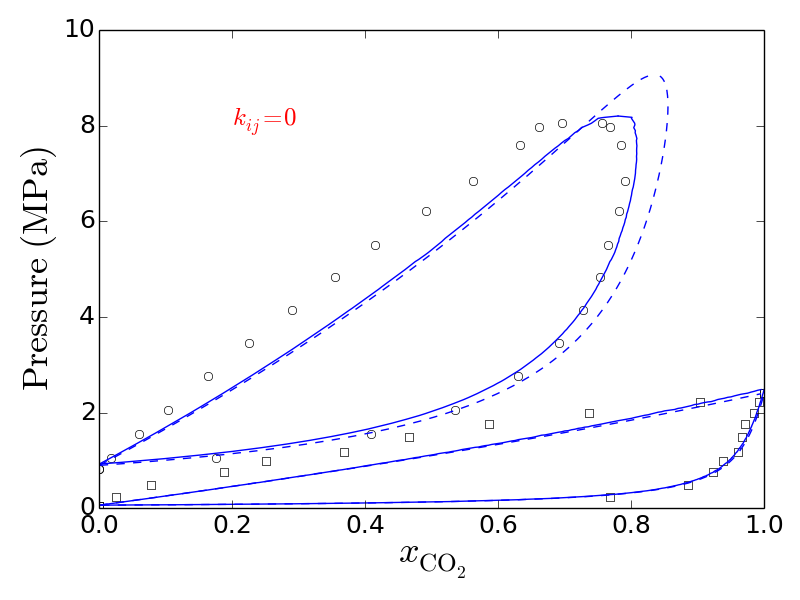
\includegraphics[width=0.75\textwidth]{figures/bin_co2_c4.png}}
\caption{vapor-liquid Phase Equilibrium Envelope to the mixture \ce{CO_2} + n-butane in the temperatures of 260K (below) and 344.3K (above).
Lines are calculated from CPA+RG(\fulline) and CPA(\dashedline).
Experimental data extracted from Clark et al.
\cite{clark1988vapour+} ($\circ$) and Hsu et al.
\cite{hsu1985equilibrium} ($\square$)}
\label{fig:bin_co2_but}
\end{figure}

\begin{figure}[h!]
\centering
\captionsetup{justification=centering}
\makebox[\textwidth][c]{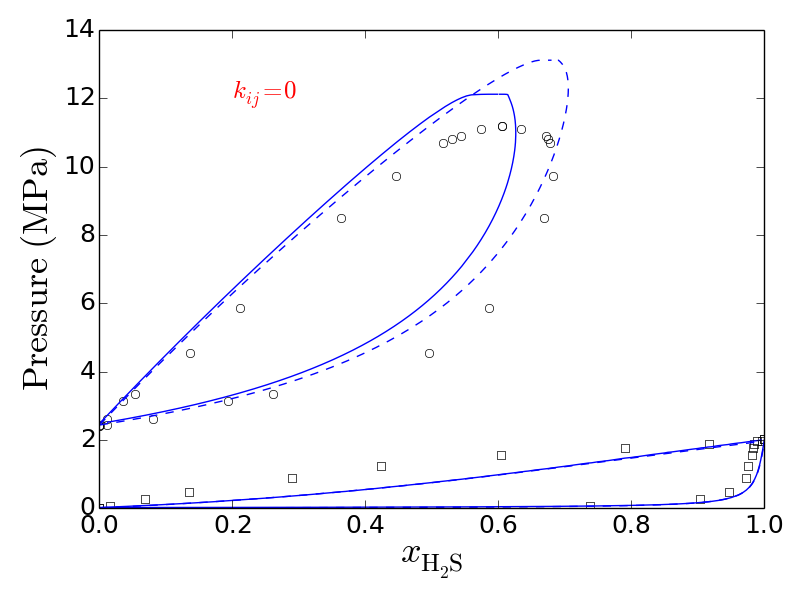
\includegraphics[width=0.75\textwidth]{figures/bin_h2s_meth.png}}
\caption{vapor-liquid equilibrium phase envelope for \ce{H_{2}S} + Methanol mixture in temperatures 298.15K (below) and 448.15K (above).
Lines are calculated from CPA+RG(\fulline) and CPA(\dashedline).
Squares Experimental data extracted from Leu et al.
 \cite{leu1992equilibrium} ($\square$,$\circ$)}
\label{fig:bin_h2s_meth}
\end{figure}

\begin{figure}[h!]
\centering
\captionsetup{justification=centering}
\makebox[\textwidth][c]{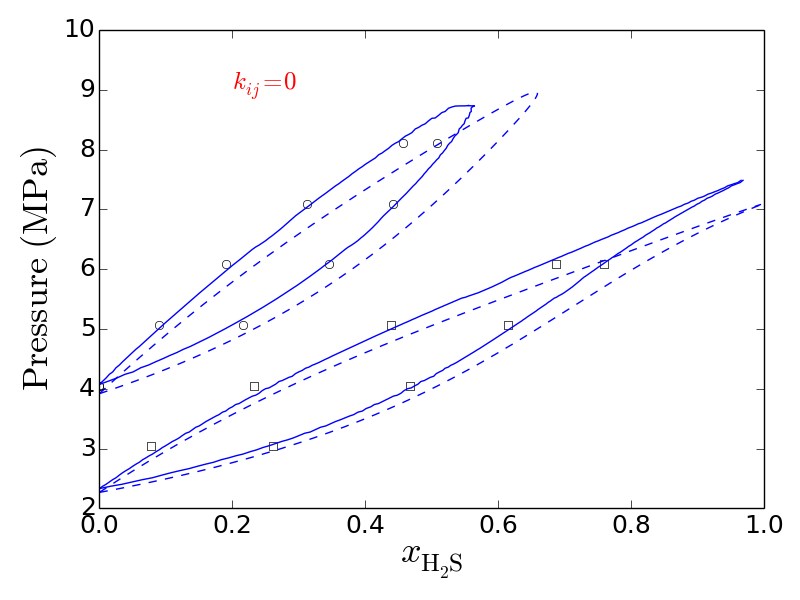
\includegraphics[width=0.75\textwidth]{figures/bin_h2s_co2.png}}
\caption{vapor-liquid equilibrium phase envelope for \ce{H_{2}S} + \ce{CO_2} mixture in temperatures 303.15K (below) and 328.15K (above).
Lines are calculated from CPA+RG(\fulline) and CPA(\dashedline).
Experimental data extracted from Bierlein et al.
 \cite{bierlein1953phase} ($\square$,$\circ$)}
\label{fig:bin_h2s_co2}
\end{figure}

Figures ~\ref{fig:bin_co2_but},~\ref{fig:bin_h2s_meth} and~\ref{fig:bin_h2s_co2} show that the renormalization method has significant influence only in the behavior of the equations of state in critical/supercritical conditions.
On correcting the fluids behavior at these conditions, the phase equilibrium representation was improved, for both dew and bubble curves.
For all evaluated mixtures the results were similar, With them, it is clear that CPA+RG approach improves the CPA equation of state behavior for binary mixtures phase equilibrium modeling.
Apparently, the difference of being an associative or non-associative component in the mixture is not an important factor for the overall result of the renormalization method.

\subsection{Derivative Properties for Pure Substances}

To assess the impact of the renormalization method on derivative properties, we calculated the isochoric heat capacity, isobaric heat capacity and speed of sound of methanol under different conditions, first as at the compressed liquid region at near-critical state, second at the critical isotherm, and finally at supercritical isotherms.
Details on the calculations are given in the Appendix C.

In the compressed liquid region, Figure~\ref{fig:cv_cp_compressed} shows that the renormalization method had no major effect on both temperatures, there is a clear tendency of increasing both heat capacities, which is better captured at lower pressures.
This effect only increases very slightly the inclination of the heat capacities curves at lower pressures.
As expected, in conditions far away from the critical point, the change is very small.

\begin{figure}[h!]
\centering
\captionsetup{justification=centering}
\makebox[\textwidth][c]{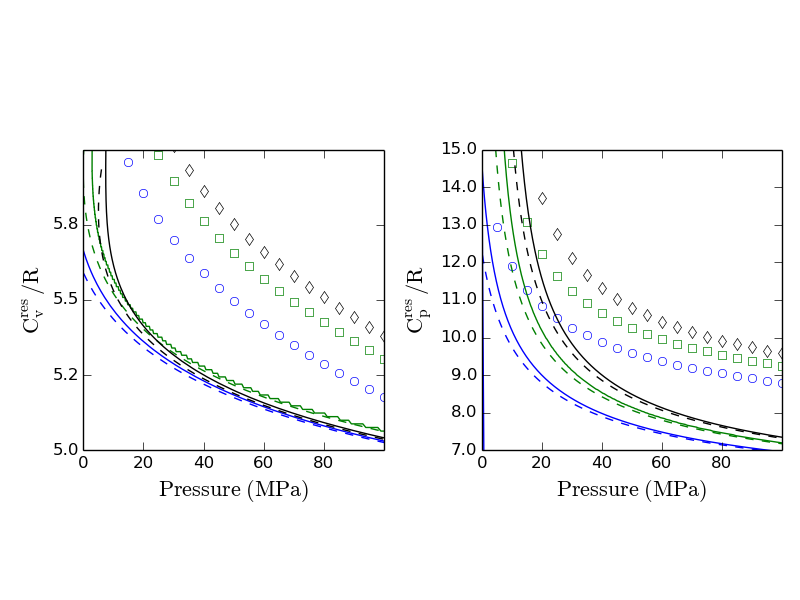
\includegraphics[width=1.0\textwidth]{figures/cv_cp_compressed.png}}
\caption{Isochoric and isobaric residual heat capacity for methanol at subcritical conditions in the compressed liquid region, symbols are experimental data from NIST database \cite{nistfluids} at T=461.34K ($\circ$), T=486.97K ($\square$) and T=507.47K ($\diamond$).
Lines are calculated from CPA+RG(\fulline) and CPA(\dashedline)}
\label{fig:cv_cp_compressed}
\end{figure}

\begin{figure}[h!]
\centering
\captionsetup{justification=centering}
\makebox[\textwidth][c]{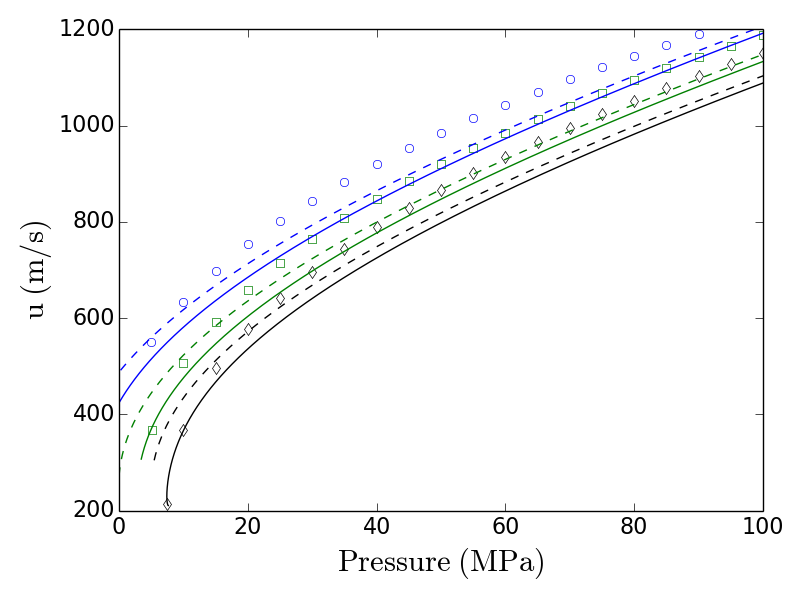
\includegraphics[width=0.65\textwidth]{figures/u_compressed.png}}
\caption{Speed of sound for methanol at subcritical conditions in the compressed liquid region, symbols are experimental data from NIST database at T=461.34K ($\circ$), T=486.97K ($\square$) and T=507.47K ($\diamond$).
Lines are calculated from CPA+RG(\fulline) and CPA(\dashedline)}
\label{fig:u_compressed}
\end{figure}

Results of speed of sound at the compressed liquid region, shown in Figure~\ref{fig:u_compressed}, shows that upon applying the renormalization method the speed of sound is very slightly decreased.
It is though, advisable to use parameters that overestimate the speed of sound.

\begin{figure}[h!]
\centering
\captionsetup{justification=centering}
\makebox[\textwidth][c]{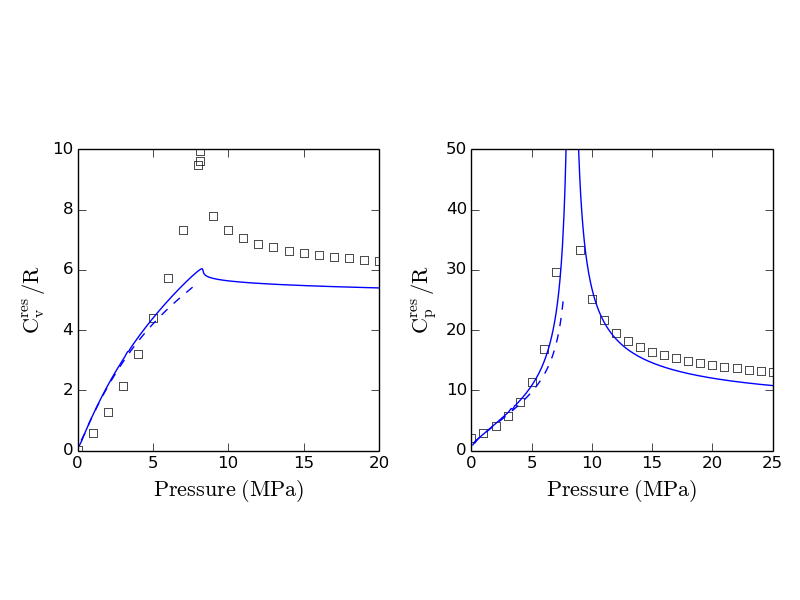
\includegraphics[width=1.0\textwidth]{figures/cv_cp_critical.png}}
\caption{Isochoric and isobaric residual heat capacity for methanol at the critical isotherm (T=512.6K).
Experimental data from NIST database \cite{nistfluids} ($\square$).
Lines are calculated from CPA+RG(\fulline) and CPA(\dashedline)}
\label{fig:cv_cp_critical}
\end{figure}

\begin{figure}[h!]
\centering
\captionsetup{justification=centering}
\makebox[\textwidth][c]{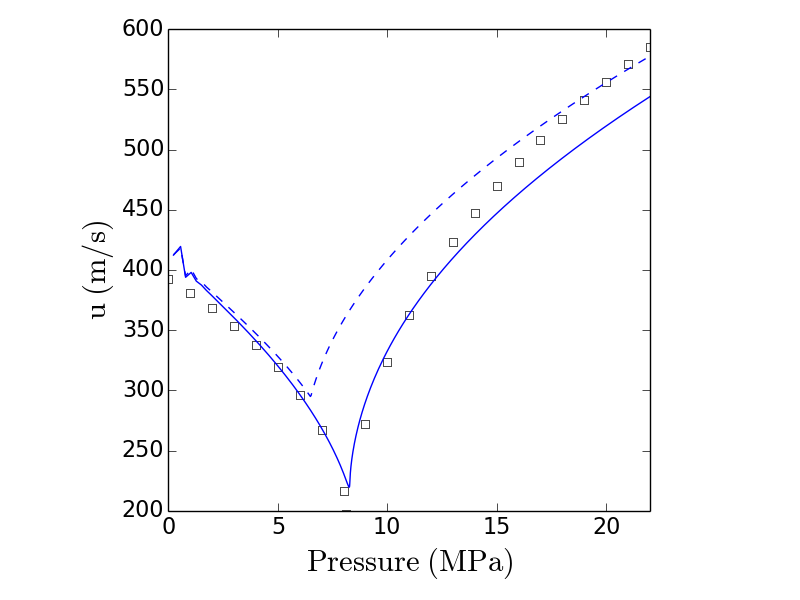
\includegraphics[width=0.65\textwidth]{figures/u_critical.png}}
\caption{Speed of sound for methanol at the critical isotherm (512.6K).
Experimental data from NIST database \cite{nistfluids} ($\square$).
Lines are calculated from CPA+RG(\fulline) and CPA(\dashedline)}
\label{fig:u_critical}
\end{figure}

At the critical temperature, both isochoric and isobaric heat capacity predictions (Figure~\ref{fig:cv_cp_critical}) are improved with the renormalization method.
The changes are more noticiable in the behavior of the curves, since the CPA equation of state is still predicting a binary phase equilibrium, while the CPA+RG approach is already predicting this condition as a near-critical/critical state.
A remarkable feature is that the renormalization method is capable of capturing the experimental critical divergence of the isobaric heat capacity, as shown in Figure~\ref{fig:cv_cp_critical}.


In the case of the speed of sound, there is a shift at the minimum of the curve when applying the renormaliation method, both in pressure and speed of sound, leaning it very near to the experimental minimum.
The prediction is better at the vicinity of this minimum, however, at higher pressures, the CPA equation of state approaches the experimental values, while the CPA+RG underestimates the experiment data.
Very peculiar results concerning the speed of sound opens a discussion on whether using speed of sound near-critical data to estimate the renormalization parameters would improve the modeling of phase equilibrium.

\begin{figure}[h!]
\centering
\captionsetup{justification=centering}
\makebox[\textwidth][c]{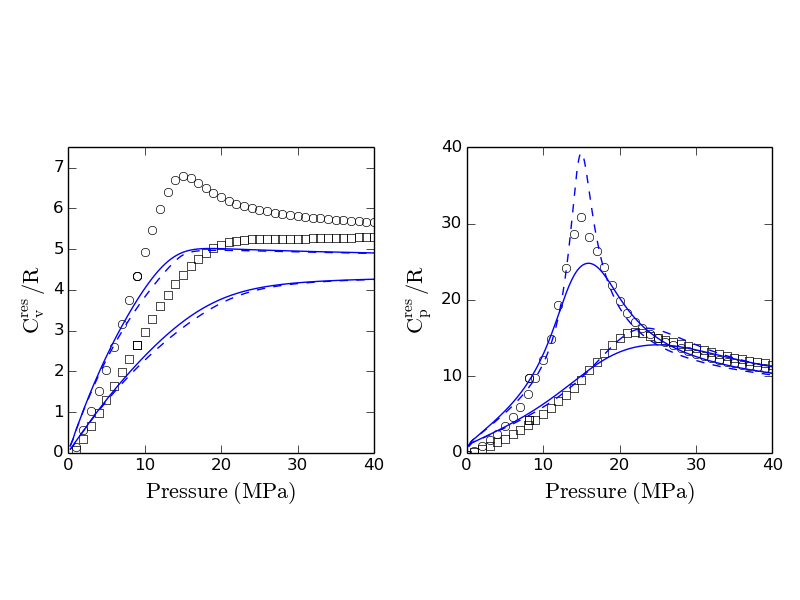
\includegraphics[width=1.0\textwidth]{figures/cv_cp_supercrit.png}}
\caption{Isochoric and isobaric residual heat capacity for methanol at supercritical isotherms, symbols are experimental data from NIST database \cite{nistfluids} at T=517.72K ($\circ$), T=538.23K ($\square$) and T=563.86K ($\diamond$).
Lines are calculated from CPA+RG(\fulline) and CPA(\dashedline)}
\label{fig:cv_cp_supercritical}
\end{figure}

\begin{figure}[h!]
\centering
\captionsetup{justification=centering}
 \makebox[\textwidth][c]{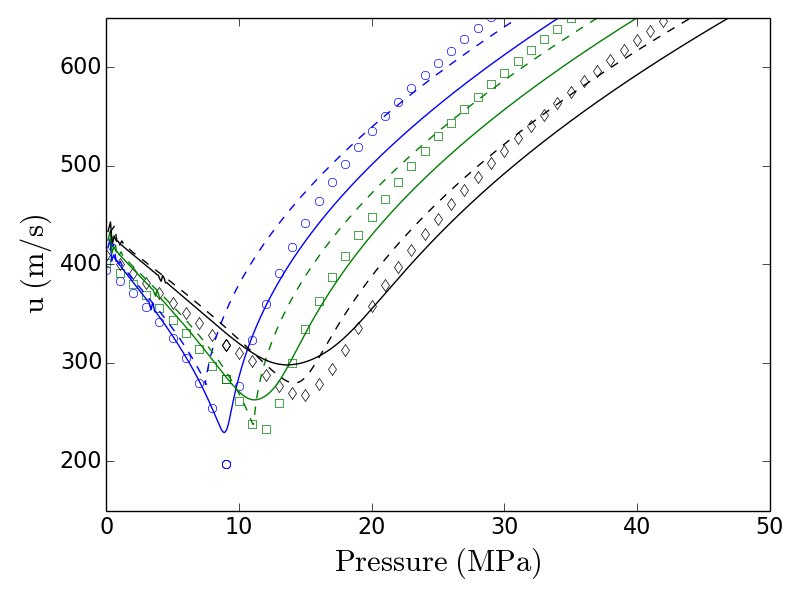
\includegraphics[width=0.65\textwidth]{figures/u_supercritical.png}}
\caption{Speed of sound for methanol at supercritical isotherms, symbols are experimental data from NIST database \cite{nistfluids} at T=517.72K ($\circ$), T=538.23K ($\square$) and T=563.86K ($\diamond$).
Lines are calculated from CPA+RG(\fulline) and CPA(\dashedline)}
\label{fig:u_supercritical}
\end{figure}

In the supercritical region, contrary to the compressed liquid region, the isobaric heat capacity has a tendency of being underestimated when the renormalization method is applied, while the isochoric heat capacity is still overestimated.
For the speed of sound results, it is clear that using the renormalization method overestimated the speed of sound near the minimum of the curve, in pressures above this point, the speed of sound was underestimated.

\section{Conclusion}

The applied methodology of renormalization group theory is capable of improving the modeling of phase equilibria in conditions near-to and at the critical point without impairing the description given by the equation of state far away from this condition.
In all cases the model behavior is improved when compared to experimental data, correcting critical exponents and introducing the expected asymptotic behavior to the fluid near the critical point.
A great advantage of the implemented method is that binary mixtures calculations do not represent computationally cumbersome tasks.
One of the major drawbacks of the method, however, is the introduction of two extra parameters.

Considering the parameter estimation, only the renormalization parameters do not guarantee improvements on the representation of $C_{p}$ and $c_{sound}$.
To model both thermodynamic properties and phase equilibrium using equations of state in conditions near-to the critical point, it may be necessary to do a parameter estimation using data from both, or even re-estimate the equation of state parameters using only data far away from the critical point.
The authors faced some problems with the used parameter estimation method, a more robust algorithm than PSO is indicated.

These results suggest that the used renormalization group methodology, together with the CPA equation of state, is a better tool than the sole CPA equation of state to describe pure acid gases and its binary mixtures phase equilibrium and derivative properties in a large range of conditions, from subcritical conditions, up to supercritical ones.

\section{Acknowledgments}
The authors would like to thank Prof.
Leo Lue for his invaluable help in providing a code to use the renormalization group method within the MSA approach, and thus allowing us to compare resuts and validate our renormalization code.
We thanks Capes, CNPQ and Petrobras for financial support.

%Making Nomenclature---------------------------------------------------
  \ifstrequal{#1}{A}{Abbreviations}{%
  
  \ifstrequal{#1}{R}{Roman Letters}{%
  
  \ifstrequal{#1}{G}{Greek Letters}{%
  
  \ifstrequal{#1}{S}{Super/subscripts}{%
  
  \ifstrequal{#1}{L}{List of Symbols}{}}}}}%

\nomenclature[A]{SRK}{Soave-Redlich-Kwong}
\nomenclature[A]{EoS}{Equation of State}
\nomenclature[A]{CPA}{Cubic-Plus-Association}
\nomenclature[A]{NIST}{National Institute of Standards and Technology}
\nomenclature[A]{RG}{Renormalization Group}
\nomenclature[A]{VLE}{Vapor-Liquid Equilibria}
\nomenclature[A]{SAFT}{Statistical Associating Fluid Theory}
\nomenclature[A]{PSO}{Particle Swarm Optimization}
\nomenclature[A]{ }{  }

\nomenclature[R]{$a$}{mixture energy parameter of equation of state}
\nomenclature[R]{$b$}{mixture co-volume parameter of equation of state}
\nomenclature[R]{$f$}{Helmholtz free energy density}
\nomenclature[R]{$\bar{a}$}{molar Helmholtz free energy}
\nomenclature[R]{$k_{ij}$}{binary interaction parameter}
\nomenclature[R]{$K$}{renormalization method coefficient}
\nomenclature[R]{$k_{b}$}{boltzmann constant}
\nomenclature[R]{$C_{v}$}{isochoric heat capacity}
\nomenclature[R]{$C_{p}$}{isobaric heat capacity}
\nomenclature[R]{$M_{w}$}{molecular weight}
\nomenclature[R]{$L$}{cutoff length}
\nomenclature[R]{$n$}{mole number}
\nomenclature[R]{$c_{sound}$}{speed of sound}
\nomenclature[R]{$v$}{molar volume}
\nomenclature[R]{$\textbf{n}$}{mole number}
\nomenclature[R]{$g$}{radial distribution function}
\nomenclature[R]{$X_{A_{i}}$}{fraction of non-bonded A site of the \textit{i}th component}
\nomenclature[R]{$u$}{pair potential}
\nomenclature[R]{$x$}{mole fraction}
\nomenclature[R]{$P$}{pressure}
\nomenclature[R]{$r$}{distance between particles}
\nomenclature[R]{$R$}{ideal gas constant}
\nomenclature[R]{$T$}{temperature}
\nomenclature[R]{$nc$}{number of components}
\nomenclature[R]{$n_{exp}$}{number of exponents}
\nomenclature[R]{ }{ }

\nomenclature[G]{$\epsilon^{A_{i}B_{j}}$}{association energy}
\nomenclature[G]{$\Delta^{A_{i}B_{j}}$}{association strength}
\nomenclature[G]{$\beta^{A_{i}B_{j}}$}{association volume}
\nomenclature[G]{$\beta$}{critical exponent}
\nomenclature[G]{$\alpha$}{interaction volume}
\nomenclature[G]{$\eta$}{packing fraction}
\nomenclature[G]{$\rho$}{molar density}
\nomenclature[G]{$\mu$}{chemical potential}
\nomenclature[G]{$\psi$}{initial shortest wavelength}
\nomenclature[G]{$\phi$}{renormalization parameter related to the initial shortest wavelength}
\nomenclature[G]{$\Omega$}{density of fluctuations}
\nomenclature[G]{ }{ }

\nomenclature[S]{pert}{perturbation}
\nomenclature[S]{ref}{reference}
\nomenclature[S]{res}{residual property}
\nomenclature[S]{assoc}{association contribution}
\nomenclature[S]{ig}{ideal gas}
\nomenclature[S]{c}{critical property}
\nomenclature[S]{0}{zero-order solution}
\nomenclature[S]{n}{\textit{n}th iteration}
\nomenclature[S]{l}{long-range}
\nomenclature[S]{liq}{liquid}
\nomenclature[S]{vap}{vapor}
\nomenclature[S]{s}{short-range}
\nomenclature[S]{exp}{experimental}
\nomenclature[S]{calc}{calculated}
\nomenclature[S]{sat}{saturated}
\nomenclature[S]{i,j}{\textit{i}th, \textit{j}th component}
\nomenclature[S]{ }{ }

\nomenclature[L]{}{}
\nomenclature[L]{}{}
\nomenclature[L]{}{}
\nomenclature[L]{}{}
\nomenclature[L]{}{}
\printnomenclature[5em]
%End Nomenclature------------------------------------------------------

\begin{appendices}
\renewcommand{\theequation}{\thesection.\arabic{equation}}
\setcounter{equation}{0}
\section{Equations and Algorithm for Phase Equilibrium Calculations for Pure Substances}
\label{app:pure substances}

After the renormalization method is applied for a given grid of density, we are left with a piece-wise curve of Helmholtz energy density.
In order to perform phase equilibrium calculations with this curve, we need to apply cubic splines interpolations.
It is advisable to use non-dimensional variables, which can be computed from its dimensional versions using the following equations (variables marked with an asterisk are non-dimensional)

\begin{equation} \label{eq:adim_dens}
\rho^{*} = \rho b
\end{equation}

\begin{equation} \label{eq:adim_T}
T^{*} = \frac{TRb}{a}
\end{equation}

\begin{equation} \label{eq:adim_f}
f^{*} = \frac{fb^{2}}{a}
\end{equation}

All derivatives can be approximated using the finite difference method, using five-point stencils for central difference.
A simple algorithm to calculate the liquid and vapor saturation densities is devised as follows:

(1) Using the equation of state, calculate the maximum liquid density ($\rho_{l,max}$) at a given temperature, with

\begin{equation} \label{eq:max_dens}
\rho^{l,max} = \frac{0.99999}{b}
\end{equation}

The 0.99999 instead of 1.00000 is used to avoid unwanted infinities.

(2) From 0 to $\rho_{l,max}$, set equally-spaced points of density (in this work we recommend using 500 points), and for each point, use the equation of state to calculate the Helmholtz free energy density

(3) For each density point in the grid, apply equations ~\cref{eq:f00,eq:fn,eq:dfn,eq:Kn,eq:Omega,eq:Gn,eq:fns,eq:fnl} for the desired number of iterations (in this work we recommend calculating 5 iterations).

(4) With the renormalization Helmholtz free energy density grid, calculate the chemical potential and pressure curves using Equations ~\ref{eq:press} and ~\ref{eq:chem_pot}

\begin{equation} \label{eq:press}
P = -f+\rho u
\end{equation}

\begin{equation} \label{eq:chem_pot}
u = \left(\frac{\partial f}{\partial \rho}\right)_{T,\textbf{n}}
\end{equation}

(5) Give liquid and vapor densities initial guesses and solve for the equilibrium conditions (equal pressure and chemical potential in both phases), calculating pressure and chemical potential using the cubic-splines interpolation.

\begin{equation} \label{eq:equal_press}
P^{vap}(\rho^{vap}) - P^{liq}(\rho^{liq}) = 0
\end{equation}

\begin{equation} \label{eq:equal_chem_pot}
\mu^{vap}(\rho^{vap}) - \mu^{liq}(\rho^{liq}) = 0
\end{equation} 

A simple newton-raphson algorithm should suffice, given that the initial guesses are consistent and far away from the trivial solution (the root at the mechanically unstable region at the pressure isotherm).
A good initial guess for the vapor density should be below the pressure of the isotherm minimum inside the coexistence curve, in the vapor region, in cases where the minimum pressure is negative, a value near zero should suffice.
The initial guess for the liquid density can be any density with a pressure higher than the isotherm maximum.
However, to solve step (5), many different algorithms can be used.

\setcounter{equation}{0}
\section{Equations and Algorithm for Phase Equilibria Calculations for Mixtures}
\label{app:mixtures}

In this work, a very usual application of the isofugacity method was used.
However, we do believe that to calculate the phase equilibria for binary or even multicomponent mixtures, very common algorithms  \cite{michelsen1982isothermal1,michelsen1982isothermal} or more recent ones '  \cite{segtovich2016simultaneous,gupta1991method} can be used, since the calculation of thermodynamic properties and variables is very straigthforward using bicubic spline interpolations.
It should be noted that the renormalization method, as it was applied, is specified in temperature, thus, applications in which the temperature is not constant may be computationally cumbersome.

As an example, an algorithm to calculate Pxy envelopes for binary mixtures is as follows:

(1) Upon specifying the temperature and molar fractions, use steps (1-3) from the procedure presented in Appendix A to obtain a renormalized Helmholtz free energy density curve

(2) Iterate over the molar fractions from 0 to 1 to obtain a renormalized Helmholtz free energy density in function of adimensional density and molar fractions.
The use of the adimensional density is what makes this step possible, since the density curve changes as the molar fractions changes.

(3) Enter the envelope calculation algorithm, interpolating the renormalized Helmholtz free energy density surface with bicubic splines to calculate the fugacity for each component from the following equations:

From the Helmholtz free energy density surface, a pressure surface can be calculated since

\begin{equation} \label{eq:press_helm_deriv}
P = -\left(\frac{\partial A}{\partial V}\right)_{T,\textbf{n}}
\end{equation}

Therefore,

\begin{equation} \label{eq:press_helm_deriv2}
P = -f+\rho\left(\frac{\partial f}{\partial \rho}\right)_{T,\textbf{n}}
\end{equation}

From the pressure-surface, with specified mole fraction, there is an isotherm in terms of pressure in function of density, from which, the densities of both phases can be calculated solving the equation:

\begin{equation} \label{eq:p_guess}
P(\rho) - P_{guess} = 0
\end{equation}

Where $P$ is calculated using the cubic spline interpolation for a given density guess.
The highest root of equation~\ref{eq:p_guess} corresponds to the liquid phase density, while the lower is the vapor phase density, good initial guesses for density could follow the pure substance algorithm.
With the densities of both phases, the residual chemical potential for the \textit{i}th component in each phase can be calculated from

\begin{equation} \label{eq:chem_pot_i}
\mu_{i}^{res} = \left(\frac{\partial f^{res}}{\partial \rho{*}}\right)_{T,x_{k\neq j,nc}}b_{i}+\sum_{j=1}^{nc} \left(\frac{\partial f^{res}}{\partial x_{j}}\right)_{T,\rho b,x_{k\neq j,nc}} \left(\frac{\delta_{ij} \rho_{i}-\rho_{j}}{\rho^{2}}\right)
\end{equation} 

Where the derivatives are calculated using the finite-difference method on the Helmholtz free energy density surface, using bicubic splines for interpolation.
Finally, to calculate fugacity, the following equation applies:

\begin{equation} \label{eq:fugacity}
ln\phi_{i} = \frac{\mu_{i}^{res}}{RT} - ln\left(\frac{P}{RT\rho}\right)
\end{equation}

With these equations, using the pressure and Helmholtz surfaces after applying the renormalization method, the fugacity coefficients can be readily calculated using bicubic spline interpolations and finite-difference derivatives.

\setcounter{equation}{0}
\section{Equations for Derivative Properties calculations}

The equations used to calculate the second derivative properties were as follows

\begin{equation} \label{eq:Cvres_deriv}
C_{v}^{res} = -T\left(\frac{\partial^{2}\bar{a}}{\partial T^{2}}\right)_{V}
\end{equation}

\begin{equation} \label{eq:Cv_deriv}
C_{v} = C_{v}^{res} + C_{v}^{ig}
\end{equation}

\begin{equation} \label{eq:Cpres_deriv}
C_{p}^{res} = C_{v}^{res} + T \left(\frac{\partial P}{\partial T}\right)_{V,\textbf{n}} \left(\frac{\partial v}{\partial T}\right)_{P}
\end{equation}

\begin{equation} \label{eq:Cp_deriv}
C_{p} = C_{p}^{res} + C_{p}^{ig}
\end{equation}

\begin{equation} \label{eq:Cvig_deriv}
C_{v}^{ig} = C_{p}^{ig} - R
\end{equation}

\begin{equation} \label{eq:u_deriv}
c_{sound} = \sqrt{\frac{C_{p}}{M_{w} C_{v}}\left(\frac{\partial P}{\partial \rho}\right)_{T,\textbf{n}}}
\end{equation}

Where $C_{p}^{ig}$ is the ideal gas heat capacity obtained from a database correlation [REF].
All derivatives are calculated using the finite-difference method with five-point-stencils.

\end{appendices}

%\bibliographystyle{ieeetr}
\bibliographystyle{elsarticle-num}
%\bibliographystyle{•}1-num-names}
\nocite{*}

\section*{\refname}

\bibliography{references}



\end{document}
